
% The general equation of a circle can be expressed as:
% \begin{align}
% \vec{x^T}\vec{x} + 2\vec{u^T}\vec{x} + f = 0 \label{4/2/15/2}
% \end{align}
% If $r$ is radius and $\vec{c}$ is the centre of the circle we have:
% \begin{align}
% f &=\vec{u}^T\vec{u}-r^2  \label{4/2/15/3} \\  
% \vec{c} &=-\vec{u} \label{4/2/15/4}
% \end{align}




% Given the point of contact $\vec{q}$, the equation of a tangent to the circle is 
% \begin{align}
% \brak{\vec{V}\vec{q}+\vec{u}}^T\vec{x}+\vec{u}^T\vec{q}+f = 0
% \label{4/2/15/5}
% \end{align}
% We know that, for a circle, 
% \begin{align}
% \vec{V} = \vec{I}  
% \end{align}



% We can rewrite \eqref{4/2/15/0} as $\vec{x}^T\vec{x} = 5$, And comparing \eqref{4/2/15/0} with \eqref{4/2/15/2}, we get
From the given information, 
\begin{align}
    \vec{c} = \vec{u}&=\myvec{0\\0},\, \vec{q}= \myvec{1\\-2}\\
    \vec{f}&=-5, r= \sqrt{5}
\end{align}
% using \eqref{4/2/15/3} and \eqref{4/2/15/4} we will get center of circle as $\vec{c} = \myvec{0\\0}$ and $r= \sqrt{5}$.
Given the point of contact $\vec{q}$, the equation of a tangent to the circle is 
\begin{align}
\brak{\vec{V}\vec{q}+\vec{u}}^T\vec{x}+\vec{u}^T\vec{q}+f = 0
\label{4/2/15/5}
\end{align}
Using \eqref{4/2/15/5},the  tangent at the point $P\myvec{1\\-2}$ is
% \begin{align}
%     \brak{\myvec{1\\-2}+\myvec{0\\0}}^T\vec{x}+\myvec{0\\0}^T\myvec{1\\-2}+{-5} = 0
% \end{align}
\begin{align}
    \implies \myvec{1&-2}\vec{x}= 5
\end{align}


The equation of the tangent line is
\begin{align}
\myvec{1&-2}\vec{x}&= 5 \label{4/2/15/a}
\end{align}

% The vector equation of a line can be expressed as 
% \begin{align}
%     \vec{x} = \vec{q} +\mu\vec{m}\label{4/2/15/c}
% \end{align}

The parameters in  \eqref{4/2/15/1} are 
\begin{align}
\vec{u}=\myvec{-4 \\ 3}, f=20
\end{align}
% If $\vec{n}$ is the normal vector of a line, equation of that line can be written as 
% \begin{align}
% \vec{n}^T\vec{x} = c \label{4/2/15/b}
% \end{align}
% Comparing \eqref{4/2/15/a} with \eqref{4/2/15/b}
\begin{align}
\vec{n} = \myvec{1 \\ -2}
\end{align}
 The point of contact $\vec{q}$, of a line with a normal vector $\vec{n}$ to the conic in \eqref{4/2/15/2} is given by:
\begin{align}
\vec{q} = \vec{V}^{-1}\brak{\kappa \vec{n}-\vec{u}} 
\\
\kappa = \pm \sqrt{\frac{\vec{u}^T\vec{V}^{-1}\vec{u}-f}{\vec{n}^T\vec{V}^{-1}\vec{n}}} 
\end{align}
% and from the properties of an Identity matrix, 
% \begin{align}
% \vec{I}^{-1} &= \vec{I} \\
% \vec{I}\vec{X} &= \vec{X}   
% \end{align}
Solving for the point of contact of \eqref{4/2/15/a} with  \eqref{4/2/15/2} using the above equations,
\begin{align}
\kappa &= \pm \sqrt{\frac{\myvec{ -4 & 3 }\myvec{-4 \\ 3} - 20}{\myvec{1 & -2 }\myvec{1 \\ -2 }}} \\
&= \pm \sqrt{\frac{25 - 20}{5}} \\
& =  \pm{1} \\
\vec{q} &= -\myvec{ 1\\-2 } - \myvec{-4 \\ 3} \\
&= \myvec{3 \\ -1}
\end{align}
% If the line in \eqref{4/2/15/c} touches \eqref{4/2/15/2} at exactly one point $\vec{q}$, then 
% \begin{align}
% \vec{m}^T\brak{\vec{V}\vec{q}+\vec{u}} = 0 \label{4/2/15/z}
% \end{align}
% It can be seen that for the given line,
% \begin{align}
% \vec{m} = \myvec{2 \\ 1} 
% \end{align}
% Solving \eqref{4/2/15/z} for given line and circle, we get
% \begin{align}
% &= \myvec{2 & 1}\brak{\myvec{3 \\ -1}+\myvec{-4 \\ 3}} \\
% &= \myvec{2 & 1}\myvec{-1 \\ 2}\\
% &= 0
% \end{align}
% And the co-ordinates of point of contact is $\myvec{3\\-1}$.
% Hence, it is proved that the tangent to the circle $\norm{\vec{x}}^2\,=\,5$ at the point \myvec{1\\-2} also touches the circle $  \vec{x}^T\vec{x}+\myvec{-8 & 6}\vec{x}+20 = 0$ at the point $\myvec{3\\-1}$.
Fig.     \ref{4/2/15/fig} verifies this result.
%
\begin{figure}[htp]
    \centering 
    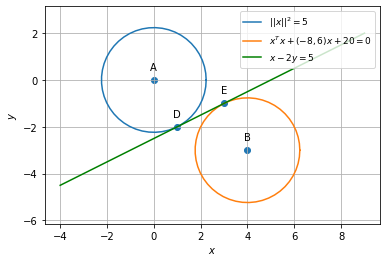
\includegraphics[width = \columnwidth]{solutions/4/2/15/a_3.png}
    \caption{Graphical illustration}
    \label{4/2/15/fig}
\end{figure}

